\setlength{\parindent}{0em}

\chapter{Umsetzung}

\label{Chapter2}

In diesem Kapitel wird näher auf die praktische Umsetzung unserer Spielidee in der Laufzeit- und Entwicklungsumgebung Unity eingegangen. Vorab sei gesagt, dass  etwaige verwendete Inhalte von Dritten in diesem Kapitel zwar namentlich genannt werden, die entsprechenden Links zu diesen allerdings erst in \textit{Kapitel \ref{Chapter4}: \nameref{Chapter4}} folgen. Dies soll der besseren Lesbarkeit und Übersichtlichkeit dienen.

%-----------------------------------
%	SPIELER-CHARAKTERE
%-----------------------------------

\section{Spieler-Charaktere}

Da unser Spiel im lokalen Multiplayer von bis zu vier Spielern gleichzeitig gespielt werden kann, besitzt unser Spiel vier verschiedene Spieler-Charaktere. Diese werden bei Spielstart in zufälliger Reihenfolge an die Mitspieler zugewiesen.\\

Abbildung~\ref{fig:player-characters} zeigt alle vier zur Verfügung stehenden Spieler-Charaktere inklusive deren jeweiliger Name im Spiel.\\

\begin{figure}[th]
\centering
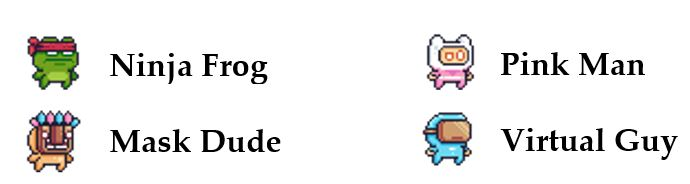
\includegraphics[width=80mm]{Figures/player-characters.jpg}
\decoRule
\caption[Spielbare Charaktere]{Spielbare Charaktere}
\label{fig:player-characters}
\end{figure}

In den nun folgenden Unterkapiteln  \ref{section: gestaltung_animation} und \ref{section: physik_bewegung} wird zunächst am Beispiel einer der vier Charaktere auf die Gestaltung und Animation sowie die Physik und Umsetzung der Bewegung eingegangen. Ebenfalls wird die \textit{InputActions}-Komponente vorgestellt, die es leicht macht verschiedene Eingabegeräte, wie Tastaturen oder Controller für das Spiel zu nutzen. In Kapitel \ref{section: player-manager} wird anschließend noch auf das von uns erstellte \textit{PlayerManager}-Prefab eingegangen, welches die Aufgabe hat, den Spielern das Beitreten zum Spiel mit ihrem jeweiligen Eingabegerät zu ermöglichen und ihnen dabei einen zufälligen, aber nicht doppelt vorkommenden Charakter zuzuweisen. Zusätzlich sorgt es dafür, dass nicht mehr Spieler beitreten können, als vor Spielstart ausgewählt wurden. Falls mindestens 2 Spieler beitreten, aktiviert es den Splitscreen, um den lokalen Multiplayer möglich zu machen.

%-----------------------------------
%	Gestaltung und Animation
%-----------------------------------
\subsection{Gestaltung und Animation}
\label{section: gestaltung_animation}

Die Grundlage für unsere Spieler-Charaktere und deren Animationen stellen die sogenannten Spritesheets des Unity-Assets \textit{Pixel Adventure 1} dar. Unter einem Spritesheet versteht man ein Bild, das mehrere kleinere Bilder enthält, die in der Regel zusammengepackt werden, um die Gesamtabmessungen zu verringern. Im Fall der Spielercharaktere benötigten wir bei allen Charakteren die  Spritesheets für die Fälle \textit{Idle (Verweilen)}, \textit{Run}, \textit{Jump} und \textit{Fall}.\\

Abbildung~\ref{fig:spritesheets_ninja} zeigt die von uns verwendeten Spritesheets am Beispiel des Charakters \enquote{Ninja Frog}.\\

\begin{figure}[th]
\centering
\includegraphics[width=150mm]{Figures/spritesheets_ninja.jpg}
\decoRule
\caption[Spritesheets des Spieler-Charakters \enquote{Ninja Frog}]{Spritesheets des Spieler-Charakters \enquote{Ninja Frog}}
\label{fig:spritesheets_ninja}
\end{figure}

Diese Spritesheets trennten wir nun zunächst mithilfe des Unity-Sprite-Editors in einzelne Sprites (Einzelbilder). Mithilfe dieser konnten wir dann für alle vier Spieler-Charaktere die jeweils benötigten Animationen erstellen. Um das Abspielen dieser Animationen gezielt steuern zu können, erstellten wir den Animator-Controller (AC) \textit{Player\_AC}. Dieser enthält zwar selbst keine sichtbaren Animationen, stellt allerdings die Logik für alle spielbaren Charaktere bereit, wann welche Animation abgespielt werden soll. Die einzelnen Charaktere wiederum besitzen einen Animator-Override-Controller (AOC) und überschreiben darin die nicht sichtbaren Animationen des Player-Animator-Controllers mit ihren spezifischen animierten Sprites. Dieser Ansatz ermöglicht es, die Logik, welche für alle Spieler-Charaktere gilt, an einer einzigen Stelle zu modifizieren und für alle wirksam zu machen.\\

Abbildung~\ref{fig:ac-aoc} zeigt den Animator-Controller \textit{Player\_AC} (links), sowie die Verwendung eines Animator-Override-Controllers am Beispiel des Charakters \enquote{Ninja Frog} (rechts).\\

\begin{figure}[th]
\centering
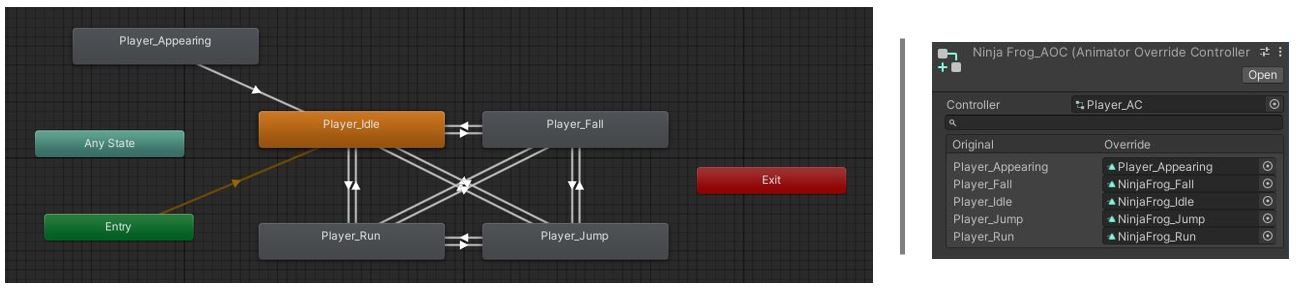
\includegraphics[width=150mm]{Figures/ac-aoc.jpg}
\decoRule
\caption[Animator-Controller und Animator-Override-Controller]{Animator-Controller (links) und Animator-Override-Controller (rechts)}
\label{fig:ac-aoc}
\end{figure}

Um im fertigen Spiel auf verschiedene Ereignisse folgend die Animation zu wechseln, wurde der Animator-Komponente \textit{Player\_AC} der Parameter \textit{state} hinzugefügt. Dieser kann vier verschiedene Integer-Werte annehmen und wechselt je nach Wert zwischen den Animationen \textit{Idle}, \textit{Run}, \textit{Jump} und \textit{Fall}. Diese Animation wird dann so lange in einer Schleife wiederholt, bis ein neuer Wert für \textit{state} gesetzt wird. Wie bei 2D-Platformern üblich wird die Animation sofort gewechselt und besitzt keine Exit-Time und keinen Übergang (Transition) der Animationen ineinander. Der Wert des Parameters \textit{state} wird im Bewegungs-Skript der Spieler-Charaktere gesetzt und in \textit{Kapitel \ref{section: physik_bewegung}: \nameref{section: physik_bewegung}} näher beschrieben.\\

Die Animation \textit{Appearing}, welche beim Spawn oder Respawn eines Spielers abgespielt wird, wird nicht über den Parameter \textit{state} gesteuert. Da diese Animation nicht in einer Schleife wiederholt werden soll, sondern nur jeweils ein einziges Mal, wird sie direkt aus dem Skript aufgerufen.\\

Da unser Spiel der Idee der etwas höheren Brutalität folgt und uns das Gegenstück zum in Abbildung~\ref{fig:spritesheets_ninja} sichtbaren Spritesheet \textit{Appear} beim Tod des Spielers nicht ausreichte, erstellten wir zusätzlich für alle Spieler-Charaktere ein Spritesheet, welches deren Körperteile im explodierten Zustand zeigt. \\

In Abbildung~\ref{fig:spritesheets_exploded} sind die von uns erstellten Spritesheets hierzu abgebildet.\\

\begin{figure}[th]
\centering
\includegraphics[width=100mm]{Figures/spritesheets_exploded.jpg}
\decoRule
\caption[Spritesheets der explodierten Spieler-Charaktere]{Spritesheets der explodierten Spieler-Charaktere}
\label{fig:spritesheets_exploded}
\end{figure}

Anders als bei den anderen Ereignissen sollten die einzelnen Sprites im Falle des Todes des Spielers natürlich nicht als Animation hintereinander angezeigt werden, sondern gleichzeitig wie bei einer Explosion in alle Richtungen davonfliegen.\\

Um dies zu erreichen, trennten wir die Spritesheets, wie oben bereits beschrieben, in ihre einzelnen Sprites und erzeugten dann aus jedem der Körperteile ein eigenes Prefab. Damit sich die einzelnen Körperteile später physikalisch korrekt verhalten, erhielten sie alle die Komponenten \textit{Rigidbody 2D} und \textit{Polygon Collider 2D}, sowie die Skripte \textit{AddForce} und \textit{SelfDestroy}. Das erstgenannte Skript sorgt dafür, dass das Körperteil direkt nach der Instanziierung im Spiel in eine zufällige Richtung weggeschleudert wird, das zweitgenannte Skript dafür, dass das Körperteil nach einer festgelegten Zeit zerstört wird und somit aus der Spielwelt verschwindet.\\

Alle Körperteile eines Spieler-Charakters zusammen dienen dann als Eingabeparameter für das ebenfalls von uns geschriebene Skript \textit{PlayerExplode}. Dieses Skript wird ausgeführt, wenn der Spieler mit einem Objekt kollidiert, welches den Tag \textit{Deadly} besitzt. Es deaktiviert die Sprite-Renderer-Komponente des Spielers, so dass dieser nicht mehr zu sehen ist, und instanziiert dann alle Körperteile in der Spielwelt an der Position des Spielers. Ebenfalls instanziiert wird das von uns erstellte Prefab \textit{BloodSplash}, welches die Komponente \textit{Particle System} verwendet, um physikalisch korrekte Blutspritzer zu erzeugen. Nach einer definierten Zeit wird der Spieler-Charakter an den nächsten Spawnpunkt gesetzt und die Sprite-Renderer-Komponente wieder aktiviert.\\

%-----------------------------------
%	Physik, Bewegung und Input Actions
%-----------------------------------
\subsection{Physik, Bewegung und Input Actions}
\label{section: physik_bewegung}

\subsubsection*{Physik}
Um es dem Spieler-Charakter zu ermöglichen, sich physikalisch korrekt durch die Spielwelt zu bewegen, fügten wir seinem Prefab die Komponente \textit{Rigidbody 2D} hinzu. Mithilfe dessen konnte dem Charakter eine Masse sowie eine Schwerkraft hinzugefügt werden. Auch kann dort durch ein Einfrieren der Rotation auf der z-Achse verhindert werden, dass der Spieler umfällt, da dies in 2D-Spielen eher unüblich ist. Die Komponente \textit{Box Collider 2D} sorgt dafür, dass der Spieler sowohl mit der Spielwelt, als auch mit anderen Objekten, wie Gegnern oder Hindernissen, kollidiert und nicht durch diese hindurch läuft oder fällt.\\

\subsubsection*{Bewegung}
Die Möglichkeit für den Charakter sich in der Spielwelt nach links und nach rechts zu bewegen, sowie zu springen und die passenden Animationen dabei abzuspielen, wird ihm durch das Skript \textit{Player Movement} gegeben, auf welches nun näher eingegangen wird.\\

Möchte der Spieler seinen Spielcharakter in der Welt bewegen und drückt auf die entsprechenden Knöpfe auf der Tastatur oder dem Controller, ruft die \textit{Input Actions}-Komponente, welche etwas später in diesem Kapitel noch näher vorgestellt wird, in dem Skript die Funktion \textit{Move(InputAction.CallbackContext context)} auf. Diese liest den übermittelten Wert für x aus dem Eingabegerät ein. Auf der Tastatur wäre dieser Wert beispielsweise \textit{1}, wenn der Spieler auf die Taste zum rechts laufen drückt und \textit{-1}, wenn der Spieler auf die Taste zum links laufen drückt. Bei einem Controller als Eingabegerät hingegen sind durch die Analogsticks auch Werte zwischen 0 und 1 bzw. -1 und 0 möglich und es kann die Geschwindigkeit des Charakters beeinflusst werden. Dieser Wert wird anschließend mit der definierbaren Variable \textit{speed} multipliziert und als neue x-Koordinate des Spieler-Objekts gesetzt. Schon bewegt sich der Spieler. Ist dieser Wert ungleich 0, ist auch klar, dass der Spieler sich bewegt und der Parameter \textit{state} des Animator-Controllers kann auf den Wert für die \textit{Run}-Animation gesetzt werden. Andernfalls wird der Wert für die Animation \textit{Idle} gesetzt. Auch kann durch diesen Wert die aktuelle Ausrichtung des Spielers geprüft werden und sich der Sprite des Spielers gegebenenfalls \enquote{flippen} lassen.\\

Ähnlich wie bei der Bewegung des Charakters auf der x-Achse funktioniert das Springen. Drückt der Spieler den entsprechenden Knopf auf der Tastatur oder dem Controller, ruft die \textit{Input Actions}-Komponente die Funktion \textit{Jump(InputAction.CallbackContext context)} auf. Innerhalb der Funktion wird durch den boolischen Wert \textit{context.performed} geprüft, ob der Knopf gedrückt wurde. Ist dies der Fall, wird die y-Koordinate des Spieler-Objekts auf die definierbare Variable \textit{jumpingPower} gesetzt. Ebenfalls Verwendung findet der boolische Wert \textit{context.canceled}. Dieser ist \textit{True}, wenn man die Taste sehr schnell wieder losgelassen hat. In diesem Fall wird die y-Koordinate nur auf die Hälfte des Wertes der Variable \textit{jumpingPower} gesetzt und das Spieler-Objekt macht nur einen halb so hohen Sprung. Damit der Spieler nicht unendlich viele Sprünge in der Luft aneinanderketten kann, ist vor jedem Sprung zu prüfen, ob der Charakter sich am Boden befindet. Hierfür verwenden wir die Methode \textit{BoxCast()} der Unity-Klasse \textit{Physics2D}. Diese gibt in unserem Fall den Wert \textit{True} zurück, wenn die \textit{BoxCollider2D}-Komponente des Spieler-Objekts die Schicht (Layer) \textit{groundLayer} berührt. Diese Schicht haben wir allen Objekten zugewiesen, von denen aus der Spieler abspringen können soll.\\

Listing~\ref{lst:player-jump} bildet die Implementierung der Jump-Funktion ab.\\

\begin{lstlisting}[caption={Funktion zur Durchführung eines Sprungs des Spielers},captionpos=b,label=lst:player-jump]
public void Jump(InputAction.CallbackContext context) {
  if (context.performed && IsGrounded()) {
    rb.velocity = new Vector2(rb.velocity.x, jumpingPower);
    GetComponent<PlayerAudioController>().PlayJumpSound();
  }
  if (context.canceled && rb.velocity.y > 0f) {
    rb.velocity = new Vector2(rb.velocity.x, rb.velocity.y * 0.5f);
  }
}
\end{lstlisting}

Die letzte Funktion, die das Skript bereitstellt, ist es, jegliche Bewegungen der Charaktere einzufrieren, bis alle in der Welt gespawnt sind. Dies verhindert, dass manche Spieler schon anfangen können, bevor alle da sind. 

\subsubsection*{Input Actions}
Die Input-Actions-Komponente von Unity ermöglicht es schnell und einfach neue Eingabegeräte für das Spiel hinzuzufügen und hilft, die logische Bedeutung einer Eingabe von den physischen Mitteln der Eingabe (also der Aktivität auf einem Eingabegerät) zu trennen. Für unser Spiel haben wir beispielsweise eine sogenannte Action Map \textit{Player} angelegt und dieser die Aktionen \textit{Move} und \textit{Jump} hinzugefügt. Diese beiden Aktionen sind alles, was der Spieler letztlich beim Spiel-Charakter steuern kann. Die Aktionen selbst kann man nun noch mit verschiedenen Eingaben verknüpfen (\textit{binding}). Abbildung~\ref{fig:input-actions} zeigt die Input Actions für unser Spiel und lässt beispielsweise erkennen, dass der Spieler die Jump-Aktion auf der Tastatur mit der Leertaste und mit einem Controller wiederum mit einem Drücken auf den sogenannten \textit{Button South} auslöst. Ebenfalls gibt es noch die Action Map \textit{UI}, welche die Aktionen zur Steuerung der grafischen Benutzeroberfläche, wie dem Haupt- und Pausenmenü, über die Tastatur oder das Gamepad enthält.\\

Wie bereits in Listing~\ref{lst:player-jump} demonstriert wurde, können ausgeführte Input Aktionen in Skripten abgefangen und ausgewertet werden.\\

\begin{figure}[th]
\centering
\includegraphics[width=150mm]{Figures/input-actions.jpg}
\decoRule
\caption[Input-Actions zur Steuerung des Spielers]{Input-Actions zur Steuerung des Spielers}
\label{fig:input-actions}
\end{figure}

%-----------------------------------
%	Player Manager
%-----------------------------------
\subsection{Player Manager}
\label{section: player-manager}

Das \textit{PlayerManager}-Objekt ist eine sehr zentrale Komponente in unserem Spiel und erfüllt mehrere wichtige Aufgaben. Zum einen hat es die Aufgabe, den Spielern das Beitreten zum Spiel mit ihrem jeweiligen Eingabegerät zu ermöglichen und ihnen dabei einen zufälligen, aber nicht doppelt vorkommenden
Charakter zuzuweisen. Zusätzlich sorgt es dafür, dass nicht mehr Spieler beitreten können, als vor Spielstart ausgewählt wurden. Falls mindestens 2 Spieler beitreten, aktiviert es den Splitscreen, um den lokalen Multiplayer zu ermöglichen. Im Folgenden wird näher auf die technische Umsetzung dieser Aufgaben eingegangen.\\

Um es überhaupt erst möglich zu machen, Spieler in einem Level spawnen zu lassen, benötigt das Objekt eine \textit{Player Input Manager}-Komponente. In dieser Komponente lässt sich festlegen, welche Eingaben auf den jeweiligen Eingabegeräten zu einer sogenannten \textit{Join Action} führen und was in diesem Fall zu tun ist. Außerdem ist ein \textit{Player Prefab} anzugeben, der dann initiiert (also gespawnt) wird. Auch kann in dieser Komponente festgelegt werden, ob der Splitscreen aktiviert wird, falls mehr als ein Spieler dem Spiel beitritt.\\

Um zu verhindern, dass jeder beitretende Spieler denselben, unter \textit{Player Prefab} angegebenen Spieler zugewiesen bekommt, implementierten wir noch das Skript \textit{CharacterSwitcher}. Dieses wird der \textit{Player Input Manager}-Komponente als Event hinzugefügt und wird ausgeführt, sobald ein Spieler beitritt. Das Skript erhält von außen eine Liste mit allen vier möglichen Spieler-Prefabs zugewiesen und bringt diese noch vor Rendern des ersten Spieleframes in eine zufällige Reihenfolge. Dann weist sie der \textit{Player Input Manager}-Komponente den ersten, nun zufälligen, Spieler-Prefab zu. Nach jedem Joint-Event weist sie der Input-Komponente das nächste Spieler-Prefab zu. Somit erhält jeder beitretende Spieler einen anderen, zufälligen Spieler-Charakter zugewiesen.\\

Um nun noch zu verhindern, dass mehr Spieler dem Spiel beitreten, als vor Spielbeginn angegeben wurde, deaktiviert das Skript \textit{PlayerManagerController} die Möglichkeit zum Beitritt, sobald die angegebene Anzahl von Spielern beigetreten ist. Außerdem wird aus diesem Skript heraus aus das Match und der Timer gestartet.\\

Abbildung~\ref{fig:player-manager} zeigt das \textit{PlayerManager}-Objekt mit all seinen Komponenten.\\

\begin{figure}[th]
\centering
\includegraphics[width=80mm]{Figures/player-manager.jpg}
\decoRule
\caption[Komponenten des \textit{PlayerManager}-Objekts]{Komponenten des \textit{PlayerManager}-Objekts}
\label{fig:player-manager}
\end{figure}

%-----------------------------------
%	Kamera und Canvas
%-----------------------------------
\subsection{Kamera und Canvas}
\label{section: camera_canvas}

Um sicherzustellen, dass jeder Spieler seinen Charakter trotz des großen Levels stets gut im Blick hat, verfügt bei uns jedes Spieler-Prefab über eine eigene Kamera-Komponente. Damit das Level auch schon angezeigt wird, bevor ein Spieler spawnt, gibt es zusätzlich noch eine Hauptkamera. Diese wird allerdings deaktiviert, sobald der erste Spieler mit seiner eigenen Kamera spawnt. Zusätzlich wurde von uns das Skript \textit{CameraFollow} geschrieben, welches dem Spieler bei seinen Bewegungen mit einem festlegbaren Offset folgt.\\

Da es auf dem Bildschirm sowohl Information darzustellen gibt, die jeden Spieler interessieren, sowie auch Informationen, die für jeden Spieler spezifisch sind und in erster Linie nur ihn betreffen, gibt es in unserem Spiel zwei verschiedene Canvas-Objekte.\\

Das erste Canvas trägt den Namen \textit{General Canvas} und befindet sich auf der obersten Ebene. Die Informationen, die sich in diesem Canvas befinden, betreffen alle Spieler gleichermaßen und überlappen entsprechend alle Spieler-spezifischen Kameras. In diesem Canvas befindet sich neben dem sogenannten \textit{Header}, bestehend aus verbleibender Zeit und einem Knopf zur Pausierung des Spiels, auch die kurze Spielerklärung, die zu Anfang jedes Levels angezeigt wird, das Pausenmenü und die Matchergebnisse.\\

Das zweite Canvas trägt den Namen \textit{Player Canvas} und befindet sich als Komponente in jedem Spieler-Prefab. Die Informationen, die sich innerhalb diesen Canvas befinden, werden jedem Spieler innerhalb seines spezifischen Splitscreens angezeigt. In unserem Spiel wird in diesem Canvas angezeigt, wie viele Punkte der Spieler bereits erreicht hat.\\

Abbildung~\ref{fig:canvas} zeigt die Bildschirmausgabe bei drei gespawnten Spielern und aktivem Pausenmenü\\

\begin{figure}[th]
\centering
\includegraphics[width=155mm]{Figures/canvas.jpg}
\decoRule
\caption[Bildschirmausgabe bei drei Spielern und aktivem Pausenmenü]{Bildschirmausgabe bei drei Spielern und aktivem Pausenmenü}
\label{fig:canvas}
\end{figure}

%-----------------------------------
%	NICHT-SPIELER-ELEMENTE
%-----------------------------------

\section{Nicht-Spieler-Elemente} 
\label{non-player-elements}

\subsection{Gegner}
Insgesamt sind im Spiel-Prototyp zum aktuellen Zeitpunkt drei verschiedene Gegnertypen implementiert, welche für den Spieler tödlich sein können. Diese werden nachfolgend jeweils kurz vorgestellt. Alle Spritesheets für die Gegner wurden dem Unity-Asset \textit{Pixel Adventure 2} entnommen.

\subsubsection*{Mushroom}

\begin{figure}[H]

\includegraphics[width=20mm]{Figures/mushroom.png}
\label{fig:mushroom}
\end{figure}

Beim Gegnertyp \textit{Mushroom} handelt es sich um kleine Pilze, welche sich in der Spielwelt auf und ab bewegen und für den Spieler tödlich sind, sollte er sie an den Seiten berühren. Dieser Gegnertyp lässt sich vom Spieler besiegen, indem dieser mittig von oben auf den Pilz springt. In diesem Fall zerspringt der Pilz in zwei Hälften und verschwindet vorerst aus der Spielwelt. Nach einer festgelegten Zeit respawnt der Pilz wieder an seiner ursprünglichen Position, um den Spielern auch im weiteren Spielverlauf eine Herausforderung zu bieten.\\

Der Sprite für den Pilz, sowie das Spritesheet für seine Laufanimation wurden dem Unity-Asset \textit{Pixel Adventure 2} entnommen. Um den Pilz bei seinem Tod ähnlich explodieren zu lassen wie die Spieler-Charaktere, wurde von uns auch hier zusätzlich ein Spritesheet mit den blutigen Hälften des Pilzes erstellt. 
Die Erstellung der Animationen, sowie die Umsetzung der Explosion des Pilzes wurden sehr ähnlich wie bei den Spieler-Charakteren umgesetzt und werden daher hier nicht noch einmal näher beschrieben. \\

Für den Pilz, sowie für weitere in Zukunft zu erstellende patrouillierende Gegner, haben wir das Skript \textit{AI Patrol} geschrieben. Dieses Skript sorgt dafür, dass die richtigen Animationen abgespielt werden und der Pilz bei nahenden Wänden oder Abgründen umdreht. Zur Erkennung von Wänden verwendet der Pilz seinen eigene \textit{Box-Collider-2D}-Komponente und überprüft ständig auf eine Kollision mit Objekten, die der Schicht \textit{groundLayer} angehören. Wird eine Kollision erkannt, so befindet sich eine Wand vor dem Pilz und dieser dreht um. Um zu erkennen, ob sich der Pilz kurz vor einem Abgrund befindet, verfügt das Pilz-Prefab zusätzlich über ein simples Transform-Objekt, welches sich etwas vor und unterhalb des eigentlichen Pilzes befindet. Auch bei diesem prüft das \textit{AI Patrol}-Skript bei jedem Frame, ob dieses Objekt ein anderes Objekt der \textit{groundLayer}-Schicht berührt. Ist dies nicht mehr der Fall, so steht ein Abgrund bevor und der Pilz dreht um.\\

Um unterscheiden zu können, wer bei einer Kollision von Spieler und Gegner stirbt und wer nicht, verfügt das Pilz-Prefab über zwei weitere \textit{Box-Collider-2D}-Objekte. Der Collider mit dem Namen \textit{SelfDeadDetect} deckt den Bereich ab, bei welchem der Pilz selbst stirbt. Wird dieser Collider vom Spieler berührt, wird das \textit{Enemy Explode} Skript getriggert und der Pilz explodiert. Der Collider mit dem Namen \textit{PlayerDeadDetect} und dem Tag \textit{Deadly} deckt den Bereich des Pilzes ab, bei welchem bei einer Kollision der Spieler stirbt. In diesem Fall wird im Spieler-Prefab das \textit{Player Explode} Skript getriggert und der Spieler explodiert.\\

Abbildung~\ref{fig:mushroom-colliders} zeigt bei beiden verschiedenen Box-Collider zur Unterscheidung der Folge eines Zusammenstoßes mit einem Spielercharakter.

\begin{figure}[th]
\centering
\includegraphics[width=70mm]{Figures/mushroom-colliders.jpg}
\decoRule
\caption[Box-Collider des Mushroom-Gegnertyps]{Box-Collider \textit{SelfDeadDetect} (links) und \textit{PlayerDeadDetect} (rechts) des Mushroom-Gegnertyps}
\label{fig:mushroom-colliders}
\end{figure}

\subsubsection*{Rhino}

\begin{figure}[H]
\includegraphics[width=25mm]{Figures/rhino.png}
\label{fig:rhino}
\end{figure}

Der Gegnertyp \textit{Rhino} ist ein Nashorn, welches aufgebracht auf einer Ebene hin und her stürmt und bei Kontakt mit einer Wand eine kurze Crash-Animation abspielt, bevor es umdreht und weiter rennt. Dieser Gegnertyp lässt sich anders als der eben beschriebene \textit{Mushroom} vom Spieler nicht besiegen, sondern ist bei jeder Berührung für den Spieler tödlich. Aus diesem Grund verfügt das Nashorn auch nur über den zusätzlichen Box-Collider \textit{PlayerDeadDetect} mit dem Tag \textit{Deadly}. Kollidiert das Spieler-Objekt mit diesem, so stirbt der Spieler.

\subsubsection*{Plant}

\begin{figure}[H]
\includegraphics[width=15mm]{Figures/plant.png}
\label{fig:plant}
\end{figure}

Der \textit{Plant} Gegner stellt eine Pflanze im Blumentopf dar, welche mit Bohnenkugeln aus ihrem Mund schießt. Dabei kann sich die Pflanze nicht von der Stelle bewegen und bildet somit ein stationäres Geschütz. Wird der Spieler von einer Bohnenkugel getroffen, ist dies tödlich für ihn. Gleichzeitig hat ein Spieler keine Chance einen Pflanzengegner zu besiegen.\\

Sowohl für die Pflanze als auch für die Bohnenkugel existieren zwei unterschiedliche Sprites, welche beide aus dem Unity-Asset \textit{Pixel Adventure 2} stammen. Das Gleiche gilt auch für die Animationen der Pflanze.\\

Als Komponenten besitzt das \textit{Prefab} der Pflanze zwei unterschiedliche \textit{Box-Collider-2D}. Einer dient als generelle Abgrenzung des \textit{GameObjects} zur Spielewelt. Der Andere hingegen fungiert als Prüfzone in welcher ermittelt wird, ob sich in dieser ein \textit{GameObject} mit dem \textit{Player}-Tag aufhält. Ist das der Fall wird die Animation der Pflanze von \textit{Idle} auf \textit{Attack} gesetzt und es werden Bohnenkugeln an der Position des Pflanzenmundes instanziiert. Tritt der Spieler aus der Prüfzone heraus, wird die Animation wieder auf \textit{Idle} gesetzt. Dies geschieht durch das \textit{Plant Logic} Skript, welches zusätzlich noch ermöglicht die Sekunden zwischen den Schüssen anzupassen. Somit ist die Feuerrate je nach Einsatzort einstellbar. Außerdem ist zu erwähnen, dass es sich bei der Bohnenkugel auch um ein eigenständiges \textit{Prefab} handelt, welches im \textit{Plant Logic} Skript referenziert wird.\\

\begin{figure}[th]
\centering
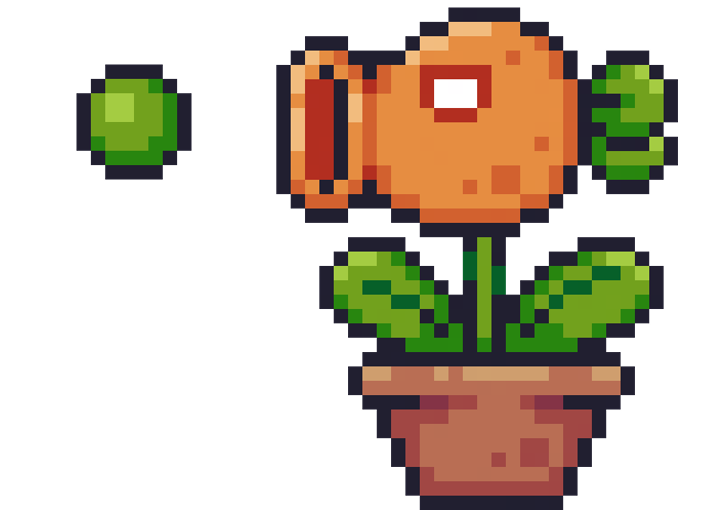
\includegraphics[width=35mm]{Figures/plant-attack.png}
\decoRule
\caption[Plant Attack Animation]{Pflanze während sie einen Schuss abgibt}
\label{fig:plant-attack}
\end{figure}

Das Bohnenkugel \textit{Prefab} besitzt das Tag \textit{Deadly} und besitzt eine \textit{Box-Collider-2D} Komponente. Somit ist diese tödlich für den Spieler, sollte er getroffen werden. Als weitere Komponente ist das eigens anfertigte \textit{Bullet Logic} Skript hinzugefügt worden. Mit diesem lassen sich Fluggeschwindigkeit und Schussdistanz einer Kugel anpassen. Außerdem ist auch in dem Skript die \textit{Destroy}-Funktion enthalten, welche das Kugel-\textit{Gameobject} zerstört, sobald es seine definierte maximale Schussdistanz erreicht.\\

\begin{figure}[th]
\centering

\includegraphics[width=75mm]{Figures/plant_idle_anim.png}
\\
\includegraphics[width=75mm]{Figures/plant_attack_anim.png}
\decoRule
\caption[Animationen der Pflanze]{Idle-Animation (oben) und Attack-Animation (unten)}
\label{fig:plant-idle-attack}
\end{figure}
\newpage
\subsection{Fallen und Hindernisse}
Insgesamt sind im Spiel-Prototyp zum aktuellen Zeitpunkt vier verschiedene Fallen- und Hindernis-Typen implementiert. Diese werden nachfolgend jeweils kurz vorgestellt. Alle Spritesheets für die Fallen und Hindernisse wurden dem Unity-Asset \textit{Pixel Adventure 1} entnommen.

\subsubsection*{Rock Head}

\begin{figure}[H]
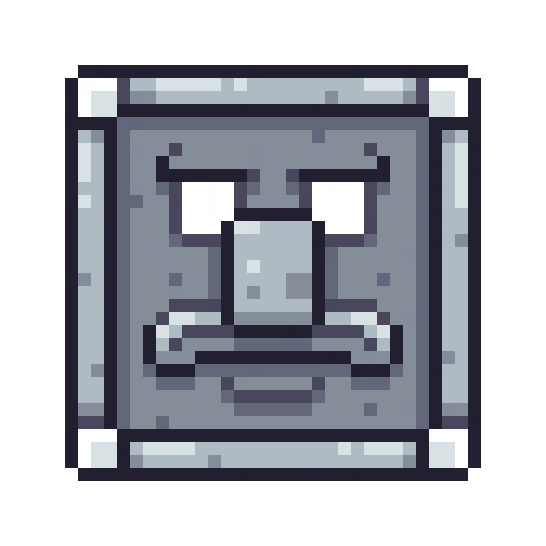
\includegraphics[width=20mm]{Figures/rock_head_idle.png}
\label{fig:Plant}
\end{figure}

Die \textit{Rock-Head}-Falle ist den fallenden Steinblöcken aus dem bekannten \textit{Super-Mario-Franchise} sehr ähnlich. Wie der Steinblock schwebt auch die \textit{Rock-Head}-Falle in der Luft, kracht zu Boden und steigt dann wieder empor, wobei sich dieser Vorgang immer wieder wiederholt. Jedoch ist es der Rock-Head-Falle möglich sich in alle vier Richtungen (unten, oben, rechts und links) zu bewegen. Wird dabei der Spieler von der Falle getroffen oder von dieser eingequetscht, ist dies für ihn tödlich. Der Spieler hat keine Möglichkeit diese Falle zu zerstören.\\

Als Komponenten besitzt die \textit{Rock-Head}-Falle einen \textit{Box-Collider-2D}, sowie das \textit{Rock Head Movement} Skript. Mit diesem wird die Beschleunigung, mit welcher sich die Falle bewegt, festgelegt. Dieser Wert wird im Skript genutzt, um die Geschwindigkeit der Falle zu berechnen. Dabei wird pro Frame die Beschleunigung auf die Geschwindigkeit aufaddiert, bis die Falle gegen ein Geländestück prallt. Anschließend wird die Geschwindigkeit auf null gesetzt. So entsteht eine natürliche Beschleunigung des Objekts.\\

Außerdem referenziert das Skript einen Array an \textit{GameObjects}. In diesem werden die Wegpunkte (\textit{engl. Waypoints}) für das Bewegungsmuster der Falle gespeichert. Mittels der \textit{MoveTowards}-Funktion der \textit{Vector2}-Klasse bewegt sich die \textit{Rock-Head}-Falle zur Position des Wegpunktes. Ist deren Position nahezu identisch, wird der nächste Wegpunkt im Array als Ziel festgelegt. Gelangt man zum letzten Index des Arrays wird die Indexvariable auf null gesetzt, um somit zu garantieren, dass die Falle ihr Bewegungsmuster immer wieder abläuft.\\

\begin{figure}[th]
\centering
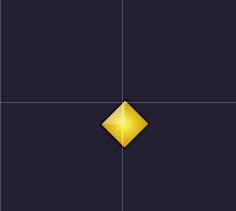
\includegraphics[width=35mm]{Figures/rock_head_waypoint.png}
\decoRule
\caption[Rock-Head-Falle Wegpunkt]{Beispiel für einen Wegpunkt einer \textit{Rock-Head} Falle}
\label{fig:rock-head-waypoint}
\end{figure}

Zusätzlich hat jedes \textit{Rock-Head-Prefab} ein \textit{PlayerDeadDetect GameObject}. Dieses definiert die Seite der Falle, welche bei Berührung tödlich für den Spieler ist. Dazu kommt eine sogenannte \textit{Deadly Zone}. Diese markiert Bereiche, in welche der Spieler sterben kann, falls er von der Falle eingequetscht wird. Dadurch ist es dem Spieler möglich die Falle als Aufzug nach oben zu verwenden. Ist dieser aber währenddessen unaufmerksam, kann er leicht von der Falle zerquetscht werden.\\

\begin{figure}[th]
\centering
\includegraphics[width=35mm]{Figures/rock_head_colli.png}
\decoRule
\caption[Rock-Head-Falle Colliders]{\textit{Rock-Head-Falle} mit dem \textit{PlayerDeadDetect GameObject} und der \textit{Deadly Zone}}
\label{fig:rock-head-collision}
\end{figure}

Die \textit{Rock-Head}-Falle besitzt fünf verschiedene Animationen. Eine \textit{Idle}-Animation, in welcher sie blinkt und vier weitere welche abgespielt werden, sobald sie gegen das Gelände in der jeweiligen Richtung aufprallt.\\

\begin{figure}[th]
\centering
\includegraphics[width=150mm]{Figures/rock_head_animator.png}
\decoRule
\caption[Rock Head Animator]{Animator der \textit{Rock-Head}-Falle}
\label{fig:rock-head-animator}
\end{figure}

\newpage

\subsubsection*{Saw}

\begin{figure}[H]
\includegraphics[width=20mm]{Figures/saw.png} 
\label{fig:saw}
\end{figure}

Es gibt zwei Einsatzformen der Sägen Falle. So gibt es eine stationäre Säge, welche an Wänden oder dem Boden angebracht werden kann und eine sich bewegende Säge. Diese kann einem vertikalen oder horizontalen Bewegungsmuster folgen, welche dem Spieler durch Verbindungsglieder einer Kette angezeigt wird. In beiden Fällen ist eine Berührung mit der Säge tödlich für den Spieler.\\

Da die stationäre Säge weniger Funktionalität benötigt, besitzt sie eine \textit{Box-Collieder-2D} Komponente und ein \textit{Rotate} Skript. Mit der Collider-Komponente wird geprüft, ob ein Spieler mit der Falle in Berührung kommt und mit dem Skript lässt sich flexibel die Geschwindigkeit, mit welcher die Säge rotiert, einstellen.\\

Neben den bereits im Prefab der stationären Säge enthaltenen Komponenten besitzt die sich bewegende Säge zusätzlich noch zwei weitere Skripte. Das \textit{WaypointFollower}- und das\textit{ChainCreator}-Skript. Bei ersterem handelt es sich um eine Abwandlung des \textit{RockHeadMovement}-Skripts. Auch hier werden leere \textit{GameObjects} als Wegpunkte referenziert, welche dann von der Säge in einer Schleife abgefahren werden. Mit dem\textit{ChainCreator}-Skript werden die Verbindungsteile der Kette instanziiert. Dabei können Werte wie die Anzahl der Verbindungsteile und der Abstand zwischen den einzelnen Teilen festgelegt werden, sowie ob die Kette horizontal oder vertikal verlaufen soll.\\

\begin{figure}[th]
\centering
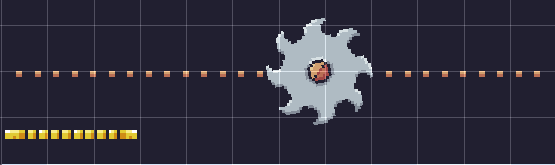
\includegraphics[width=120mm]{Figures/saw-with-chain.png}
\decoRule
\caption[Bewegliche Sägen Falle]{Sich bewegende Sägen-Falle mit Kette}
\label{fig:saw-with-chain}
\end{figure}

\subsubsection*{Fallende und sich bewegende Plattformen}

\begin{figure}[H]
\includegraphics[width=20mm]{Figures/falling platform.png}
\quad
\includegraphics[width=20mm]{Figures/platform.png}
\label{fig:platforms}
\end{figure}

Beide Plattformen stammen aus dem \textit{Pixel Adventure 1} Assetpaket, besitzen aber verschiedene Eigenschaften. Die in Abbildung~\ref{fig:platforms} links dargestellte Plattform stellt eine Falle für den Spieler dar. Diese fällt nach Berührung mit dem Spieler nach kurzer Zeit zu Boden und kann so für unaufmerksame Spieler tödlich sein. Die rechte Plattform hingegen bietet dem Spieler eine Transportmöglichkeit über vertikale und horizontale Distanzen.\\

Der \textit{Prefab} der sich bewegenden Plattform besitzt die \textit{Box-Collider-2D} Komponente, welche es dem Spieler ermöglicht sich auf die Plattform zu stellen. Damit dieser während der Fahrt der Plattform nicht hinunterfällt implementierten wir das \textit{Sticky Platform} Skript. Durch dieses wird die Position des Spielers während einer Kollision mit der Position der Plattform synchronisiert. Entfernt sich der Spieler wieder von der Plattform, setzt sich seine Position zurück. Um das Bewegungsmuster der Plattform zu definieren, schrieben wir das \textit{WaypointFollower}-Skript, welches eine Abwandlung des \textit{RockHeadMovement}-Skripts ist, welches wir für die Bewegungsmuster der Steinblock Gegner verwenden. Auch hier werden leere \textit{GameObjects} als Wegpunkte referenziert, welche dann von der Plattform in einer Schleife abgefahren werden.\\

\begin{figure}[th]
\centering
\includegraphics[width=120mm]{Figures/platform-example.png}
\decoRule
\caption[Fahrt eines Spieler-Charakters auf einer Plattform]{Spieler auf einer sich bewegenden Plattform}
\label{fig:platform-example}
\end{figure}

Das \textit{Prefab} der fallenden Plattform besitzt neben der \textit{Box-Collider-2D} Komponente auch die \textit{Rigidbody-2D}-Komponente, welche es ermöglicht einem \textit{GameObject} physische Attribute zu geben. Diese Attribute werden mit dem eigens angefertigten \textit{FallingPlatform} Skript manipuliert. Tritt der Spieler auf die Plattform wird nach einer definierbaren Zeit die \textit{DropPlatform}-Funktion ausgeführt, welches das \textit{Rigidbody} Attribut \textit{isKinematic} des \textit{GameObjects} auf \textit{false} setzt und es somit zu Boden stürzen lässt und dann zerstört wird. Nach einer ebenfalls definierbaren Zeit erscheint die Plattform erneut.\\

\begin{lstlisting}[caption={Logik der fallenden Plattform},captionpos=b]
private void OnCollisionEnter2D(Collision2D other){
    if (other.gameObject.CompareTag("Player")){
        Invoke("DropPlatfrom", timeToDrop);
        GetComponentInParent<ObjectRespawnerController>()
        .RespawnObject(spawnPosition, respawnDelay);
        Destroy(gameObject, timeToDelete);
    }
}
private void DropPlatfrom(){
    rb.isKinematic = false;
}
\end{lstlisting}

\newpage

\subsubsection*{Spikes}

\begin{figure}[H]
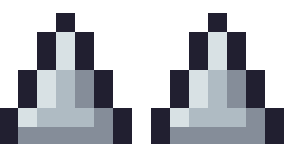
\includegraphics[width=20mm]{Figures/spikes.png}
\label{fig:spikes}
\end{figure}

Bei den Spikes handelt sich um ein Fallen-Objekt, welches den Spieler bei einer Kollision tötet und im fertigen Spiel an sehr vielen Stellen dafür sorgt, dass bestimmte Fehler des Spielers überhaupt erst eine tödliche Konsequenz haben. Beispielsweise lässt sich damit erreichen, dass das Herunterfallen von Plattformen oder das ungenaue Springen eines Spielers durch an Böden, Decken und Wänden angebrachten Spikes den Spieler tötet und ihm somit eine größere Herausforderung bietet. Auch werden die Spikes teilweise verwendet, um bestimmte Bereiche für den Spieler unzugänglich zu machen. Im Level werden die einzelnen Spikes zu Spike-Sets zusammengefasst und diese jeweils mit einer \textit{Box-Collider-2D}-Komponente und dem Tag \textit{Deadly} versehen. Bei einer Kollision des Spielers mit einem Objekt mit dem Tag \textit{Deadly} wird dann das Skript \textit{Player Explode} innerhalb des Spieler-Objekts ausgeführt und der Spieler explodiert.

\subsection{Sammelbare Früchte}

\begin{figure}[H]
\includegraphics[width=17mm]{Figures/apple.png}
\includegraphics[width=20mm]{Figures/cherry.png}
\includegraphics[width=20mm]{Figures/pineapple.png}
\label{fig:fruits}
\end{figure}

Die drei verschiedenen Früchte – ein Apfel, eine Kirsche und eine Ananas – sind die einzigen vom Spieler aufsammelbaren Gegenstände im Spiel. Dabei besitzt jede Frucht eine unterschiedlich hohe Punkteanzahl.

\begin{itemize}
\item Apfel = 1 Punkt
\item Kirsche = 2 Punkte
\item Ananas = 5 Punkte
\end{itemize}

Diese Punktzahl dient als Entscheidungswert dafür, welcher der Spieler das Spiel letztlich gewinnt. Diese Punktzahl wird während des gesamten Spiels über dem jeweiligen Spieler angezeigt. Die Sprites stammen aus dem Unity-Assetpaket \textit{Pixel Adventure 1}.\\

Jedes der Früchte \textit{Prefabs} besitzt einen \textit{Box-Collider-2D}. Dies ermöglicht uns die \textit{OnTriggerEnter2D}-Methode, um damit zu prüfen, ob das \textit{GameObject} mit dem Spieler kollidiert. Ist das der Fall wird die \textit{Collected}-Animation abgespielt.Nachdem diese abgespielt ist, wird das \textit{GameObject} per \textit{Destroy}-Methode zerstört.\\

\begin{figure}[th]
\centering
\includegraphics[width=150mm]{Figures/apple_collected.png}
\decoRule
\caption[Animation des Apfels beim Aufsammeln durch den Spieler]{Animation des Apfels beim Aufsammeln durch den Spieler}
\label{fig:apple-collected}
\end{figure}
\newpage
%----------------------------------------------------------------------------------------
%	LEVELGESTALTUNG
%----------------------------------------------------------------------------------------

\section{Levelgestaltung}

Bei der Levelgestaltung verwendeten wir neben den von uns erzeugten Objekten aus \textit{Kapitel \ref{non-player-elements} \nameref{non-player-elements}} zusätzlich noch diverse allgemeine Terrain-Spritesheets aus dem Unity-Asset \textit{Pixel Adventure 1}, beispielsweise für Böden, Wände und den Hintergrund. Diese zerlegten wir wieder mithilfe des Unity-Sprite-Editors in ihre einzelnen Sprites und fügten diese einer sogenannten Tile-Palette hinzu. Aus dieser heraus lässt sich relativ bequem der statische Teil des Levels und der Hintergrund zusammenbauen.\\

Abbildung~\ref{fig:tile-palette} zeigt die von uns verwendete Tile-Palette für die Terraingestaltung und den Hintergrund.\\

\begin{figure}[th]
\centering
\includegraphics[width=80mm]{Figures/tile-palette.jpg}
\decoRule
\caption[Verwendete Tile-Palette für das Terrain den Hintergrund]{Verwendete Tile-Palette für das Terrain und den Hintergrund}
\label{fig:tile-palette}
\end{figure}

Aufgrund des benötigten Umfangs bei einem Level, welches von bis zu vier Spielern gleichzeitig bespielt werden soll, umfasst unser Spiel bisher nur ein Level. Dieses ist allerdings auch entsprechend groß. Im folgenden Kapitel soll dieses Level kurz vorgestellt werden.

\subsection{Level 1}

Im ersten Level unseres Spiels finden sich alle von uns implementierten Fallen, Hindernisse und Gegner wieder. Diese sind so im Level platziert und teilweise aneinandergereiht, dass sie dem Spieler eine möglichst große Herausforderung bieten. Die Items, die die Spieler sammeln, müssen um Punkte zu bekommen, sind so verteilt, dass nach besonders schwierigen Passagen wertvollere Items auf den Spieler warten, als in leichten Passagen. Bei der Erstellung des Levels wurde besonders darauf geachtet, dass die einzelnen Bereiche in keiner Sackgasse enden und der Spieler nicht den ganzen Weg zurück gehen muss. Außerdem wird so sichergestellt, dass die Spieler die Bereiche von beiden Seiten betreten können und sich keine Nachteile aus dem Spawnpunkt des Spielers ergeben. Die vier Spawnpunkte selbst sind so gesetzt, dass die Spieler direkt nach dem ersten Spawnpunkt möglichst weit weg voneinander sind und sich nicht gegenseitig behindern.\\

Abbildung~\ref{fig:level1} zeigt die Ausmaße des ganzen Levels in der Szenenansicht von Unity.

\begin{figure}[th]
\centering
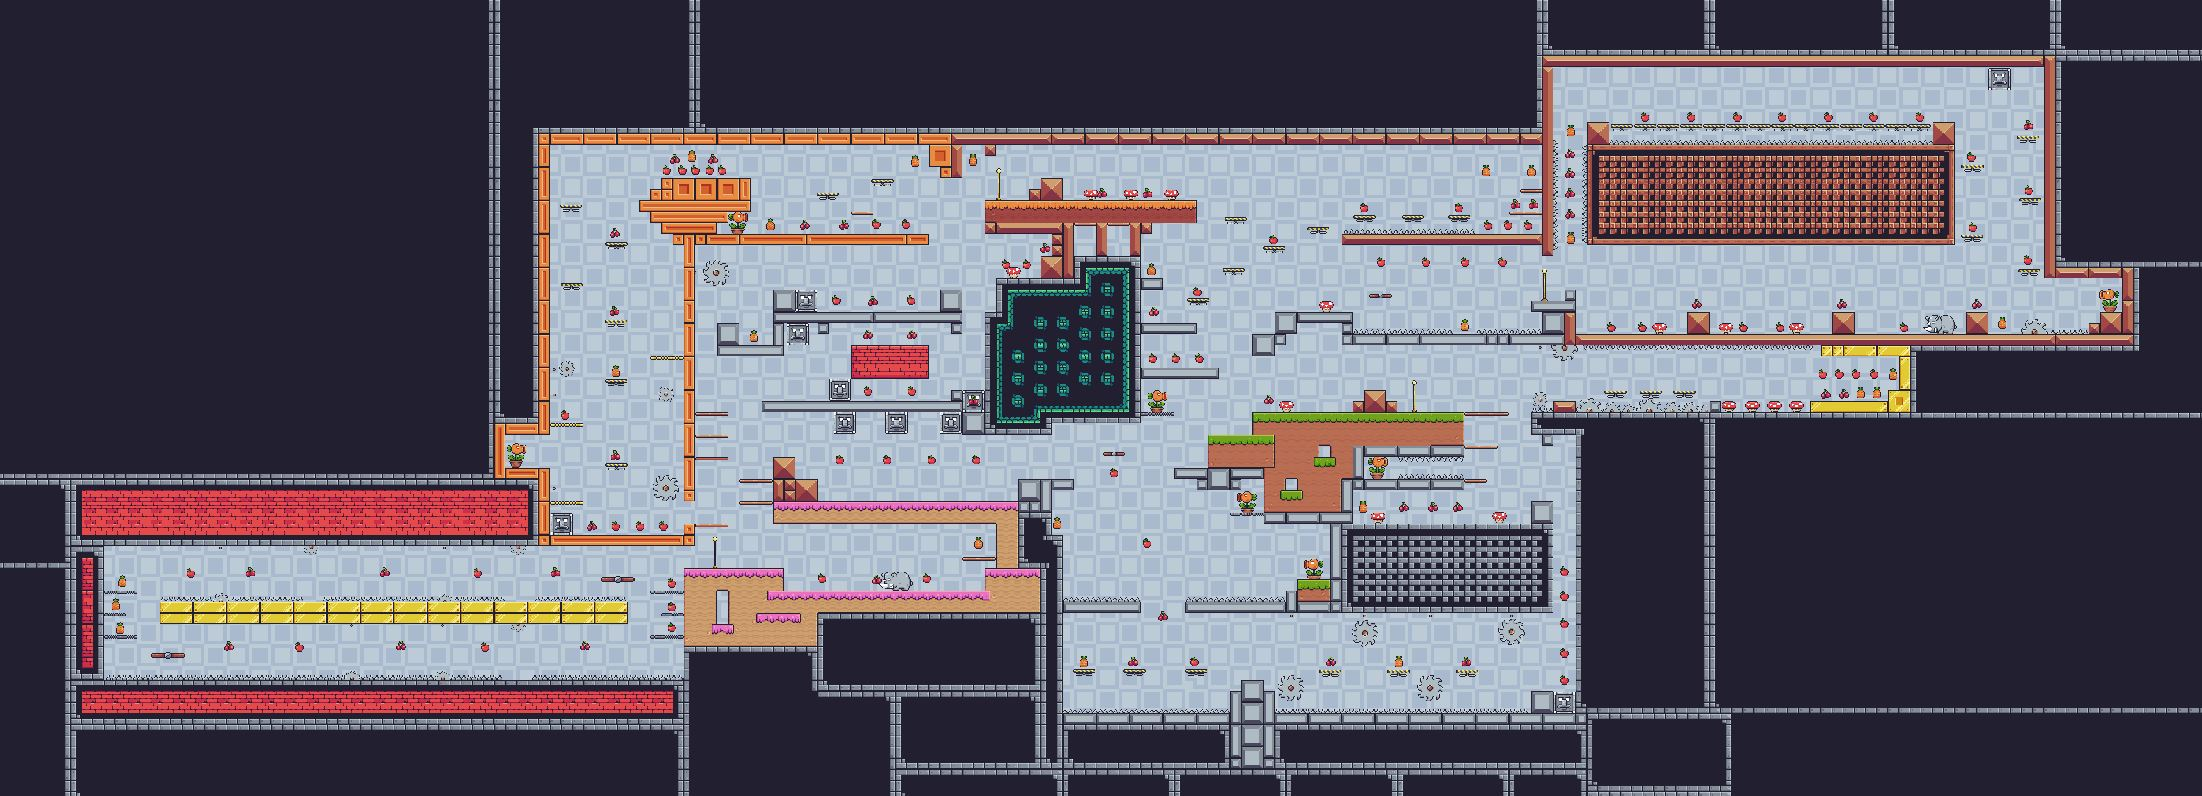
\includegraphics[width=155mm]{Figures/level1.jpg}
\decoRule
\caption[Übersicht über das ganze 1. Level]{Übersicht über das ganze 1. Level}
\label{fig:level1}
\end{figure}

%-----------------------------------
%	GRAFISCHE BENUTZEROBERFLÄCHE
%-----------------------------------

\section{Grafische Benutzeroberfläche}

%----------------------------------------------------------------------------------------
%	HAUPTMENÜ
%----------------------------------------------------------------------------------------
\subsection{Hauptmenü}
Für das Hauptmenü haben wir in Unity eine eigene Szene erstellt und ein eigenes kleines Minilevel erstellt, welches durch herumlaufende Gegner, sowie den animierten Helden des Spiels dafür sorgen soll, dass das Hauptmenü nicht so statisch und langweilig wirkt. Die Anzeige der Schaltflächen befinden sich in einem Canvas-Objekt und wird an einer Stelle angezeigt, an der sie das Mini-Level nicht überdeckt. Je nachdem auf welche Schaltfläche der Spieler drückt, werden nach Bedarf Schaltflächen ausgeblendet und andere Schaltflächen angezeigt.\\

Da uns keine der Standard-Schriftarten von Unity überzeugt hat, haben wir uns für die Aufschriften auf den Schaltflächen, sowie den Namen des Spieltitels eine lizenzfreie Schriftart aus dem Internet gesucht. Nach Umwandlung der Schriftart in ein \enquote{TextMeshPro}-Asset konnten wir die Schriftart zusätzlich in Unity weiter bearbeiten und so beispielsweise einen froschgrünen Schatten hinzufügen. \\

Um die getroffenen Einstellungen für die Lautstärke und die Rundenezeit unter \enquote{Settings} auch nach einem Neustart des Spiels beibehalten zu können, haben wir die Unity-Klasse \enquote{PlayerPrefs} verwendet, welche die Werte im Plattform-Register des Benutzers speichert.\\

Bedienen lässt sich das Hauptmenü und das im nächsten Kapitel beschriebene Pausenmenü sowohl mit der Maus, als auch mit der Tastatur oder dem Gamepad. Das aktuell ausgewählte Objekt ist hierbei immer etwas dunkler dargestellt, um die Bedienung zu erleichtern.\\

Abbildung~\ref{fig:15Ai} zeigt das Hauptmenü direkt nach Starten des Spiels.\\

\begin{figure}[th]
\centering
\includegraphics[width=150mm]{Figures/main-menu.jpg}
\decoRule
\caption[Hauptmenü]{Hauptmenü nach Starten des Spiels}
\label{fig:main-menu}
\end{figure}

%----------------------------------------------------------------------------------------
%	PAUSENMENÜ
%----------------------------------------------------------------------------------------
\subsection{Pausenmenü}
Um das Spiel während der Spielrunde anzuhalten oder die Runde neu zu starten respektive zu beenden, lässt sich mit einem Klick auf das \enquote{Pause}-Symbol neben der verbleibenden Rundenzeit (oder der entsprechenden Taste auf Tastatur oder Gamepad) das Pausenmenü öffnen. Während das Pausenmenü geöffnet ist, ist die Variable timeScale der Unity-Klasse Time auf 0 gesetzt und das Spielgeschehen somit angehalten. Schließt der Spieler das Pausenmenü, wird die Variable wieder auf 1 gesetzt und das Spiel wird dort fortgesetzt, wo es gestoppt wurde. Vom Pausenmenü aus kann der Spieler die Runde auch neu starten oder beenden.\\

Abbildung~\ref{fig:pause-menu} zeigt eine angehaltene Spielrunde mit geöffnetem Pausenmenü.\\

\begin{figure}[th]
\centering
\includegraphics[width=150mm]{Figures/pause-menu.jpg}
\decoRule
\caption[Pausenmenü]{Geöffnetes Pausenmenü während einer Spielrunde}
\label{fig:pause-menu}
\end{figure}

%----------------------------------------------------------------------------------------
%	MATCH-RESULTAT
%----------------------------------------------------------------------------------------
\subsection{Match-Resultat}
Sobald die Rundenzeit abgelaufen ist, werden durch die in Listing~\ref{lst:calc_player_results} gezeigte Methode die Statistiken der Spieler ausgewertet und die Spieler ihrer Leistung nach sortiert. Bei dieser Berechnung sind die erreichten Punkte des Spielers am wichtigsten. Bei selber Punktzahl wird derjenige besser platziert, der weniger Tode hatte. In dem unwahrscheinlichen Fall, dass Spieler dann immer noch gleich auf sind, wird alphabetisch sortiert. Die errechnete Platzierung wird dann an die Methode FillRow der Komponente Leaderboard übergeben, welche die Daten in die jeweiligen Zeilen einträgt. Ist dies geschehen, wird das Fenster, welches das Match-Resultat beinhaltet gerendert.\\

Abbildung~\ref{fig:match-results} zeigt ein Match-Resultat nach einem Spiel mit zwei Spielern.\\

\begin{lstlisting}[caption={Funktion zur Berechnung der Spielerplatzierungen},captionpos=b,label=lst:calc_player_results]
void CalculatePlayerScores() {
  List<GameObjec> players = new List<GameObject>(GameObject.FindGameObjectsWithTag("Player"));
  players = players.OrderByDescending(
            p=>p.GetComponent<PlayerStats>().points)
            .ThenBy(p=>p.GetComponent<PlayerStats>().deaths)
            .ThenBy(p=>p.name)
            .ToList<GameObject>();
    
  for (int i = 0; i < placesAmount; i++) {
    if (placesAmount < players.Count) {
      lbPlaces[i].GetComponent<Leaderboard>().FillRow(players[i]);
    } else {
      lbPlaces[i].GetComponent<Leaderboard>().FillRow(null);
    }
  }
}
\end{lstlisting}

\begin{figure}[th]
\centering
\includegraphics[width=150mm]{Figures/match-results.jpg}
\decoRule
\caption[Match-Resultat]{Match-Resultat nach einem Spiel mit 2 Spielern}
\label{fig:match-results}
\end{figure}

%----------------------------------------------------------------------------------------
%	SOUND-GESTALTUNG
%----------------------------------------------------------------------------------------

\section{Sound-Gestaltung}

%----------------------------------------------------------------------------------------
%	SOUNDEFFEKTE
%----------------------------------------------------------------------------------------
\subsection{Soundeffekte}

\subsubsection*{Im Spielgeschehen}
Da unser Spiel im lokalen Multiplayer im Splitscreen von bis zu vier Spielern gleichzeitig gespielt werden kann, haben wir uns bewusst dazu entschlossen, die Anzahl und die Lautstärke der Soundeffekte möglichst zu begrenzen. Wir haben etwa die Geräusche beim Laufen der Spieler und Gegner sowie die Geräusche von verschiedenen Hindernissen nachträglich wieder entfernt, da diese bei einer höheren Spieleranzahl ständig zu hören waren und genervt haben. Die Lautstärke beim Springen der Spieler haben wir beibehalten, aber drastisch in der Lautstärke reduziert. Soundeffekte von Ereignissen, die nicht so oft auftreten, wie etwa das (Re-)Spawnen der Spieler, das Einsammeln eines Items oder die Explosion von Spielern oder Gegnern bei deren Tod, haben wir unverändert beibehalten. Um allerdings auch dort etwas Abwechslung zu garantieren, rufen manche Ereignisse einen zufälligen Soundeffekt aus einer bestimmten Gruppe auf. So wird bei der Explosion eines Spielers oder Gegners beispielsweise zufällig einer von drei verfügbaren blutigen Explosionsgeräuschen abgespielt. Beim Aufsammeln von Items entscheidet die Wertigkeit des Items über den abgespielten Sound. Je wertiger das Item ist, desto effektvoller ist der Soundeffekt.

\subsubsection*{In der Benutzeroberfläche}
Auch die grafische Benutzeroberfläche im Haupt- und Pausenmenü verfügt über Soundeffekte. Diese beschränken sich allerdings auf das Abspielen eines Geräuschs beim Betätigen eines Buttons bzw. beim Loslassen eines Sliders.

%----------------------------------------------------------------------------------------
%	KOMMENTATOR-SPRÜCHE
%----------------------------------------------------------------------------------------
\subsection{Kommentator-Sprüche}
Um das Spiel weiter von einem üblichen Jump-n-Run-Spiel abzuheben, haben wir einen Kommentator implementiert, welcher je nach aktuellem Geschehen verschiedene Kommentare über den Spieler und
das Spielgeschehen abgibt. Dabei ist der Kommentator dem Spieler allerdings nicht sehr wohlgesonnen, sondern kritisiert den Spieler hauptsächlich auf zynisch-spöttische Art. Da die meisten Text-To-Speech-Systeme weder menschlich klingen, noch die passenden Stimmlagen für dieses Vorhaben anbieten oder die gewünschten Emotionen in der Stimme herüberkommen lassen, haben wir uns nach einer frei verfügbaren, KI-getriebenen Sprachsynthese-Technologie umgesehen und sind bei der Webanwendung unter \url{https://15.ai/} fündig geworden.\\

In der Webanwendung lässt sich aus diversen Charakteren aus der Film- und Spielwelt auswählen und nach Eingabe eines Textes verschiedene Sprachausgaben erzeugen. Durch die Angabe von Emotionen hinter dem auszusprechenden Text lässt sich auch ein direkter Einfluss auf die Stimmlage und -betonung nehmen. Abbildung~\ref{fig:15Ai} zeigt die Verwendung des Tools am Beispiel des Zeichentrick-Charakters SpongeBob Schwammkopf.\\

\begin{figure}[th]
\centering
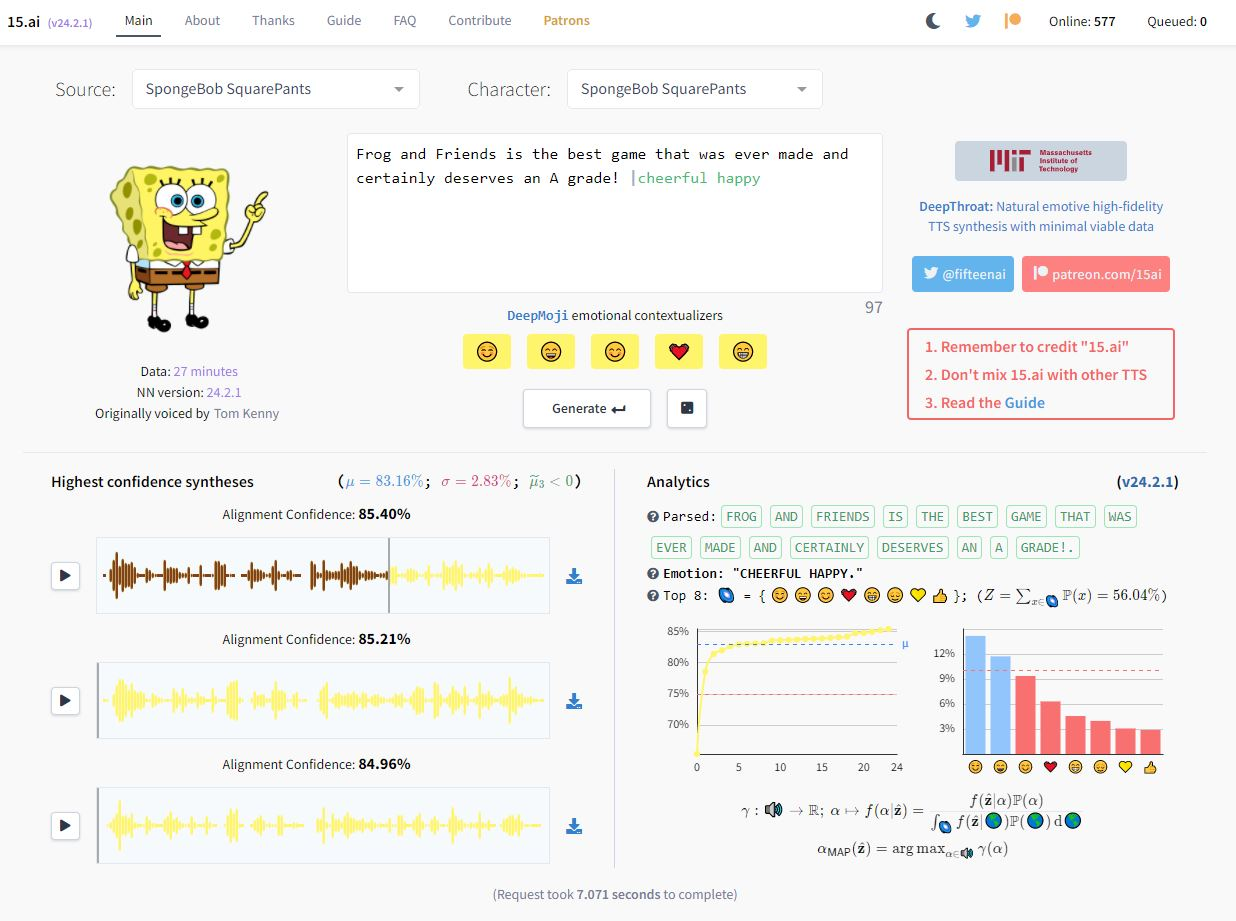
\includegraphics[width=150mm]{Figures/15AI.jpg}
\decoRule
\caption[Verwendung der Webanwendung 15.ai zur Sprachsynthese]{Verwendung der Webanwendung zur Sprachsynthese unter \url{https://15.ai/}}
\label{fig:15Ai}
\end{figure}

Da wir für den Kommentator nach einer sehr lauten, tiefen Stimme gesucht haben, haben wir als Stimmquelle den Charakter \enquote{Heavy} aus dem Videospiel \enquote{Team Fortress 2} gewählt.
Insgesamt haben wir uns für den Kommentator über 70 Sprüche ausgedacht, sie generiert, heruntergeladen und ins Spiel integriert.
Dabei kommentiert der Kommentator das Spiel in folgenden Situationen:

\begin{itemize}
 \item Das Level wird gestartet
 \item Verbleibende Spielzeit erreicht bestimmte Marke
 \item Der Spieler stirbt
 \item Der Spieler sammelt ein Item ein (verschiedene Sprüche für verschiedene Itemtypen)
 \item Der Spieler tötet einen Gegner
 \item Das Level ist zu Ende und die Ergebnisse und Spielerplatzierungen werden angezeigt
\end{itemize}

Neben den Kommentator-Sprüchen haben wir auch für die einzelnen spielbaren Charakter noch jeweils eine Audiodatei generiert, in welcher sie ihren eigenen Namen ausrufen.
Dieser Ausruf findet pro Spieldurchgang allerdings nur einmal statt, wenn der jeweilige Charakter zum ersten Mal im Level gespawnt wird. Die hierfür verwendeten Stimmenprofile setzen sich folgendermaßen zusammen:

\begin{itemize}
 \item \enquote{Ninja Frog}: Demoman (Team Fortress 2)
 \item \enquote{Virtual Guy}: Tenth Doctor (Doctor Who)
 \item \enquote{Mask Dude}: Dan (Dan Vs.)
 \item \enquote{Pink Man}: SpongeBob SquarePants (SpongeBob SquarePants)
\end{itemize}

%----------------------------------------------------------------------------------------
%	HINTERGRUNDMUSIK
%----------------------------------------------------------------------------------------
\subsection{Hintergrundmusik}
Bei der Hintergrundmusik, welche im Hauptmenü und den einzelnen Levels läuft, haben wir uns bewusst für Musikstücke entschieden, die durch ihre fröhliche, heitere Art in einem
kompletten Gegensatz zur für das Spielgenre unüblichen Brutalität des Spiels und dem spöttischen Spiel-Kommentator stehen.
So soll das Spiel mit seiner grafischen und musikalischen Aufmachung zunächst an ein kindgerechtes, buntes Plattformer-Spiel erinnern und sich dem Spieler das wahre Gesicht des Spiels erst während des eigentlichen Spielens offenbaren.\\

Insgesamt verfügt das Spiel über vier verschiedene Musikstücke, welche durch ein Skript zufällig nacheinander abgespielt werden. Die Grundlautstärke der Hintergrundmusik ist deutlich leiser angesetzt, als die von Soundeffekten oder den Sprüchen des Kommentators, um diese nicht zu überschatten. Wie alle anderen Audioeffekte kann die Lautstärke der Hintergrundmusik im Hauptmenü verändert werden. 
